\documentclass[assignment3.tex]{subfiles}
\begin{document}

\section*{1η Άσκηση}
%\begin{figure}[hp]
%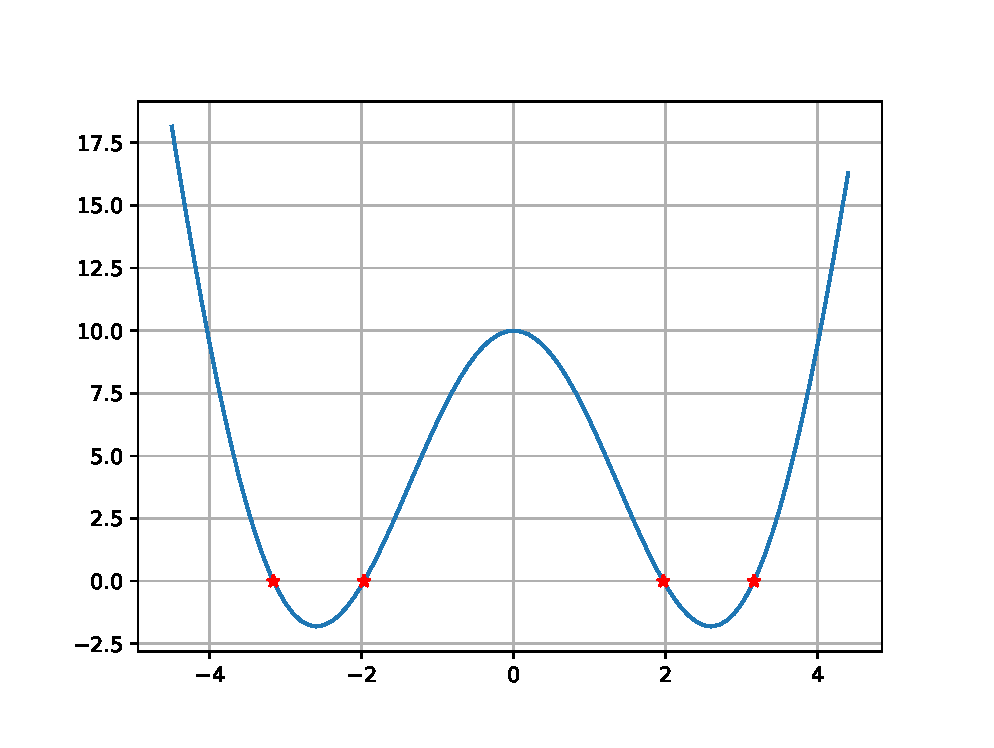
\includegraphics[width=0.7\textwidth]{f1.eps}
%\centering
%\caption{Γράφημα $x^2+10\cos x$ γύρω από το $O(0,0)$}
%\label{fig:f1}
%\end{figure} 



%\begin{table}[ht]
%\centering
%\begin{tabular}{||c c c||} 
%	\hline
%	$g_i$& $\rho>0$ & $\rho<0$ \\ [0.5ex] 
%	\hline\hline
%	$\arccos \left(-\frac{x^2}{10}\right)$ & 1.9689 & -1.9689 \\ 
%	\hline
%	$\sqrt{-10\cos x}$ & 3.1619 & -3.1619 \\ [1ex] 
%	\hline
%\end{tabular}
%\caption{Αποτελέσματα Προσομοίωσης}
%\label{table:fixed_point}
%\end{table}

%Παρακάτω ακολουθεί ο κώδικας που γράφτηκε σε \textlatin{Python} και έγινε χρήση της βιβλιοθήκης \textlatin{Numpy}. Ο αλγόριθμος της μεθόδου σταθερού σημείου δίνεται στο Παράρτημα.
%\selectlanguage{english}
%\lstinputlisting[style=python, firstline=8]{ex1.py}
\end{document}